\section{Лестницы ширин в размерностях 2--6}
\label{sec:ladders}

Метод даёт не только оценки на $\chi(\R^n)$, но и раскраски, запрещающие целый
отрезок расстояний. Здесь собраны такие результаты: компромисс
<<цвета\,$\leftrightarrow$\,ширина>> в $\R^4$, точный оптимум семейства
$G(\alpha)$ в $\R^3$ и лестницы ширин в $\R^3$, $\R^5$, $\R^6$.

\subsection{Более широкий интервал в $\R^4$: $45$, $46$ и $48$ цветов}
\label{ssec:wide45}

Оценка $\chi(\R^4)\le43$ работы~\cite{Bounds} рекордна по числу цветов, но её
интервал узок ($\ell\le1{,}00411$). Для более широких запрещённых интервалов
лучшими остаются решётки \emph{общего положения} --- они не эйзенштейновы и в
трёхпараметрическое семейство решётки $43$ не попадают. Чемпион индекса~$45$:
$\Lambda_{45}=B^{\mathsf T}\Z^4$ с
\begin{equation}\label{eq:gram}
Q=\begin{pmatrix}
\tfrac{91}{15}  & \tfrac{29}{16} & -\tfrac{51}{11} & -\tfrac{55}{12}\\[3pt]
\tfrac{29}{16}  & \tfrac{123}{10}& -\tfrac{19}{4}  & -\tfrac{73}{15}\\[3pt]
-\tfrac{51}{11} & -\tfrac{19}{4} & 16              & -\tfrac{7}{5}\\[3pt]
-\tfrac{55}{12} & -\tfrac{73}{15}& -\tfrac{7}{5}   & \tfrac{139}{9}
\end{pmatrix}
\qquad(7920\,Q\in\mathrm{Mat}_4(\Z)),
\end{equation}
и подрешёткой индекса~$45$ с переходом
\begin{equation}\label{eq:hnf}
T=\begin{pmatrix}1&0&0&15\\0&1&0&41\\0&0&1&37\\0&0&0&45\end{pmatrix},
\qquad\det T=45 .
\end{equation}
Здесь $\lambda_1^2=\tfrac{91}{15}$, $\diam^2V_0\approx23{,}451$,
$D^2\approx24{,}223$, $d=1{,}016339\ldots$; ячейка имеет $30$ фасет и
$f$-вектор $(120,240,150,30)$, у $\Lambda_{45}$ \emph{единственная} пара
кратчайших векторов, $2R/\lambda_1\approx1{,}966$, и она не изометрична ни
одной классической решётке ($D_4$, $A_4^*$, $\Z^4$, $A_4$).

При индексе~$48$ та же оптимизация даёт заметно большую ширину. Для рациональной
решётки с матрицей Грама
\[
Q_{48}=\begin{pmatrix}
\tfrac{137}{12}&\tfrac{13}{7}&-\tfrac{61}{10}&-\tfrac{18}{5}\\[2pt]
\tfrac{13}{7}&7&-\tfrac{25}{9}&-\tfrac{37}{12}\\[2pt]
-\tfrac{61}{10}&-\tfrac{25}{9}&12&-\tfrac{17}{11}\\[2pt]
-\tfrac{18}{5}&-\tfrac{37}{12}&-\tfrac{17}{11}&\tfrac{44}{5}
\end{pmatrix}
\]
и подрешётки индекса~$48$ с наддиагональю $(28,16,30)$ в последнем столбце
получается $d=1{,}039657677\ldots$ (здесь $\lambda_1^2=7$,
$\diam^2P=19{,}141641$, $D^2\ge20{,}689971$).

\begin{keybox}
\begin{theorem}\label{thm:main}
$\chi\bigl(\R^4,[1,\ell]\bigr)\le45$ при всех $1\le\ell\le1{,}015$, и
$\chi\bigl(\R^4,[1,\ell]\bigr)\le48$ при всех $1\le\ell\le1{,}0396$.
\end{theorem}
\end{keybox}
\begin{proof}
Точные сертификаты неравенств $d>\ell_0$ для обеих форм ---
файлы \path{audit-data/results/cert45.json} и
\path{audit-data/results/cert48.json}; схема проверки --- протокол точного
сертификата статьи~\cite{Bounds} в опорной форме: объемлющий многогранник
$P\supseteq V_0$ с рациональными вершинами даёт $\diam V_0\le\diam P$
сверху и $\dist(v/2,V_0)\ge\dist(v/2,P)$ снизу для каждого вектора
подрешётки в доказуемо полном окне, и итоговое неравенство
$D^2\ge\ell_0^2\diam^2P$ проверяется в дробях.
\end{proof}

Три ступени вместе:
\[
\begin{array}{lccc}
\text{цветов} & 43 & 45 & 48\\
\ell\le & 1{,}00411 & 1{,}015 & 1{,}0396\\
\text{решётка} & \text{эйзенштейнова~\cite{Bounds}} & \text{общего положения} & \text{общего положения}
\end{array}
\]
Итак, увеличив число цветов на пять ($43\to48$), можно расширить запрещённый
интервал почти вдесятеро ($1{,}00411\to1{,}0396$) --- этот компромисс
<<цвета${}\leftrightarrow{}$ширина>> ранее не отмечался. Ширина здесь ---
расходуемый ресурс (предложение~\ref{prop:product}), поэтому в
произведениях блок с $45$ цветами полезнее блока с $43$: $1/1{,}015^2=0{,}971$
оставляет запас бюджета, а $1/1{,}00411^2=0{,}9918$ --- практически нет.

Таблица~\ref{tab:r4} собирает все четыре полученные решёточные раскраски
$\R^4$: рекордную по числу цветов ($43$) и три с более широким запрещённым
интервалом ($45$, $46$, $48$). У всех четырёх ячейка Вороного имеет $f$-вектор
$(120,240,150,30)$ --- такой же, как у четырёхмерного пермутоэдра, --- и
подрешётку с циклической матрицей перехода; для каждой доказан точный
сертификат $d>\ell_0$. Решётка индекса~$43$ эйзенштейнова, остальные три ---
общего положения. Матрицы Грама для $k=45$ и $48$ выписаны выше, для $k=43$ ---
в \cite{Bounds}, для $k=46$ --- в файле \path{audit-data/results/cert46.json}.

\begin{table}[h]
\centering
\caption{Решёточные раскраски $\R^4$: $\chi(\R^4,[1,\ell])\le k$ при
$\ell\le\ell_0$. Столбец <<знам.>> --- наибольший знаменатель рациональной
матрицы Грама; <<$d$ (числ.)>> --- ширина численного оптимума; десятичные
значения <<$d$ (рацион.)>> округлены вниз.}
\label{tab:r4}
\small
\begin{tabular}{c c c c c l}
\toprule
$k$ & $\ell_0$ (сертиф.) & $d$ (рацион.) & $d$ (числ.) & знам. & примечание\\
\midrule
\textbf{43} & $\mathbf{1{,}00411}$ & $1{,}004110$ & $1{,}004112$ & $10^5$
  & \textbf{рекорд по числу цветов}; эйзенштейнова~\cite{Bounds}\\
45 & $1{,}015$ & $1{,}016339$ & $1{,}017401$ & $16$ & общего положения\\
46 & $1{,}004$ & $1{,}005068$ & $1{,}005405$ & $24$ & промежуточный\\
48 & $1{,}0396$ & $1{,}039657$ & $1{,}043270$ & $12$ & наибольший интервал\\
\bottomrule
\end{tabular}
\end{table}

\subsection{Лестницы ширин и семейство $G(\alpha)$ в $\R^3$}\label{sec:stair}

Дешёвая оценка формы Грама без полного перебора подрешёток
(полная версия~\cite{Full}, \S3) позволяет строить \emph{лестницы ширин}
и в старших размерностях: при большем числе цветов запрещённый интервал
расширяется (на фиксированной $A_5^*$ до $[1,\,1{,}265]$ при $k=300$,
табл.~\ref{tab:stair56}). При $n\ge7$ запрещённое множество быстро растёт
($|F_1|\approx1{,}9\cdot10^4$ для $A_7^*$,
${\approx}3{,}5\cdot10^4$ для $E_7$), поэтому сплошной перебор индексов
становится дорогим и поиск ведётся по \emph{курируемым} индексам.

Рис.~\ref{fig:stair} показывает <<лестницы>> максимальной ширины $d(k)$ ---
бегущий максимум по классическим решёткам --- для $\R^2$, $\R^3$, $\R^4$. Порог
$d=1$ впервые достигается при $k=7$ (шестиугольная решётка, $\R^2$), $k=15$
(ОЦК, $\R^3$) и $k=49$ по классическим решёткам в $\R^4$ (решётки общего
положения опускают его до~$45$, эйзенштейновы --- до~$43$~\cite{Bounds}).

\begin{figure}[t]
\centering
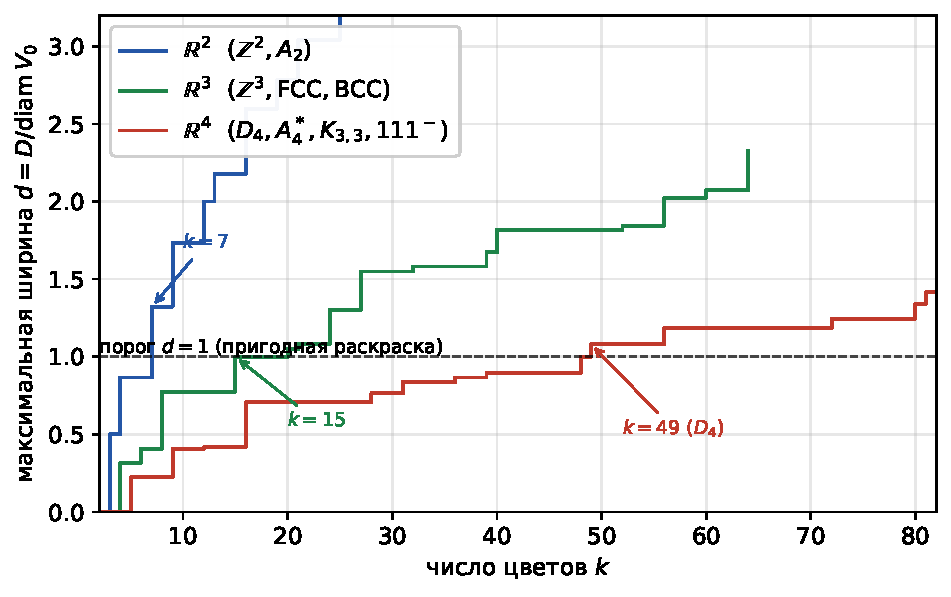
\includegraphics[width=0.74\textwidth]{fig_staircase.pdf}
\caption{Максимальная нормированная ширина $d(k)$ как функция числа цветов $k$
для $\R^2$, $\R^3$, $\R^4$ (бегущий максимум по классическим решёткам каждой
размерности). Пунктир --- порог $d=1$: правее точки пересечения раскраска в $k$
цветов правильна для классического расстояния.}
\label{fig:stair}
\end{figure}

\paragraph{Размерность 3: оптимальность 15 цветов и расширение интервала.}
В отличие от $\R^4$, в $\R^3$ число цветов уменьшить нельзя: по теореме
Кулсона \cite[теорема~4.5]{Coulson} (см. также \cite{ABPR}) решёточная
раскраска $\R^n$ требует не менее $2^{n+1}-1$ цветов, так что
$\chi_s(\R^3)\ge15$ и $15$ цветов --- оптимум среди решёточных раскрасок
$\R^3$. Наш поиск с этим согласуется: оптимизация метрики при
$k=8,\dots,14$ ни разу не достигает порога $d=1$ (максимум $d=0{,}900$ при
$k=14$), а оболочечный экран \S\ref{sec:floors} даёт ту же границу $15$ на
фиксированном родителе ОЦК независимо от теоремы Кулсона
(теорема~\ref{thm:a3opt}).

Исторически первая решёточная $15$-раскраска предложена Кулсоном
\cite{Coulson}; её родительская решётка --- ОЦК ($A_3^*$). Рассмотрим её
внутри однопараметрического семейства форм
\[
G(\alpha)=\begin{pmatrix}1&-\alpha&2\alpha-1\\-\alpha&1&-\alpha\\
2\alpha-1&-\alpha&1\end{pmatrix},
\qquad
T=\begin{pmatrix}1&0&11\\0&1&7\\0&0&15\end{pmatrix},
\]
где матрица перехода $T$ подрешётки индекса~$15$ \emph{фиксирована}, а при
$\alpha=1/3$ форма пропорциональна ОЦК --- это случай Кулсона. Решение
KKT-систем связывающих орбит в замкнутой форме даёт
\[
D^2_{(3,2,2)}=\frac{4\alpha^2+3\alpha+1}{\alpha+1},\qquad
D^2_{(2,1,-1)}=\frac{2(5\alpha^2-6\alpha+2)}{1-\alpha},\qquad
\diam^2 V_0=2-\alpha,
\]
и семейство оказывается достаточно широким, чтобы покрыть \emph{обе}
конструкции работы~\cite{Coulson}.

При $\alpha=1/3$ ширина равна \emph{ровно} $1$ (проверено и полным точным
аудитом: $12$ векторов окна, все KKT-сертификаты): интервал вырожден, и
предложение~\ref{prop:crit}, требующее строгого $\ell<d$, к этой точке
неприменимо --- оценка $\chi(\R^3)\le15$ получена в \cite{Coulson} отдельным
разбором границ ячеек. Но в конце работы \cite{Coulson} приведена
\emph{улучшенная} $15$-раскраска уже с невырожденным исключённым интервалом
расстояний $\bigl(\sqrt{22},\ \sqrt{389/17}\bigr)$, то есть после нормировки
$\bigl(1,\ \sqrt{389/374}\bigr)$, где
$\sqrt{389/374}=1{,}0198563\ldots$ Оба этих числа в точности воспроизводит
точка $\alpha=4/13$ нашего семейства: замкнутые формы дают там
$\diam^2 V_0=22/13$ и $D^2_{\min}=389/221$, то есть при масштабе~$13$ ---
ровно кулсоновские $22$ и $389/17$, а полный точный аудит ($8$ векторов окна)
подтверждает $d^2=389/374$. Совпадают оба рациональных инварианта, поэтому
улучшенная раскраска \cite{Coulson} --- почти наверное именно эта точка
семейства (само отождествление решёток мы не проверяли: в \cite{Coulson}
ячейка задана рисунком).

Максимум семейства достигается там, где связывающая ветвь меняется, ---
разность ветвей факторизуется точно,
\[
D^2_{(3,2,2)}-D^2_{(2,1,-1)}
=\frac{14\alpha^3-3\alpha^2-10\alpha+3}{(\alpha-1)(\alpha+1)},
\]
так что $\alpha^*$ есть корень кубики $p(x)=14x^3-3x^2-10x+3$. Вещественных
корней у неё три, поэтому нужный задаётся \emph{рациональным изолирующим
окном}: $3136953/10^7<\alpha^*<3136954/10^7$. Корень там есть, поскольку
$p$ меняет знак на концах, и он единствен: $p''(x)=84x-6>0$ на окне, а
$p'(3136954/10^7)<0$, значит $p'<0$ на всём окне и $p$ строго убывает. Это
точное задание алгебраического числа, а с ним точна и ширина:
\[
(d^*)^2=\frac{4\alpha^{*2}+3\alpha^*+1}{(\alpha^*+1)(2-\alpha^*)}
=\frac{602\alpha^{*2}-87\alpha^*+143}{166},
\qquad d^*=1{,}0265985838\ldots
\]
(вторая запись --- редукция по кубике). Лучший найденный численный оптимум по
всем шестипараметрическим формам ($1{,}0265930$) его не превосходит, так что
семейство $G(\alpha)$, по-видимому, содержит глобальный оптимум $k=15$.

Отсюда строгая рациональная граница, без всякой плавающей точки. Обозначим
через $r_A(x)=(4x^2+3x+1)/\bigl((x+1)(2-x)\bigr)$ квадрат ширины на ветви
$(3,2,2)$; его производная равна
$r'_A(x)=(7x^2+18x+5)/\bigl((x-2)^2(x+1)^2\bigr)$ и при $x\ge0$ положительна
(корни числителя отрицательны), поэтому $r_A$ возрастает и
$(d^*)^2=r_A(\alpha^*)>r_A(3136953/10^7)$, а одно точное вычисление в дробях
даёт
\[
r_A\Bigl(\tfrac{3136953}{10^7}\Bigr)-\Bigl(\tfrac{102659}{100000}\Bigr)^2
=\frac{38\,881\,620\,997\,802\,732\,729}
{2\,215\,290\,558\,757\,910\,000\,000\,000}>0 .
\]
Полный сертификат ставится в рациональной точке $\alpha=3137/10000$
(целочисленный грамиан $10^4G$), отстоящей от $\alpha^*$ на
$4{,}7\cdot10^{-6}$: $14$ фасет, $24$ вершины, окно $\|v\|<2(1+\ell)R$ из
$12$ векторов, KKT-сертификат каждого --- вся цепочка в точной арифметике
дробей, $d^2=121967690/115730769$, и
\begin{keybox}
\[
\chi\bigl(\R^3,[1,\ell]\bigr)\le15\qquad
\Bigl(\ell\le\tfrac{102659}{100000}=1{,}02659\Bigr)
\]
\end{keybox}
\noindent --- точный рациональный сертификат. Запрещённый интервал шире
кулсоновского на $0{,}66\,\%$; у Кулсона обоснование геометрическое, здесь ---
конечный список неравенств между явно выписанными дробями, проверяемый
независимой программой. Сертификат --- все четыре точки семейства
($\alpha=1/3$, $4/13$, $3137/10000$ и прежняя $16/51$) вместе с рациональной
границей для $\alpha^*$ --- \path{audit-data/results/dim3_k15_certificate.json}.

При $k>15$ оптимизация метрики по всему пространству форм заметно улучшает
прежнюю таблицу \cite{Ivanov2011} для $\R^3$ (табл.~\ref{tab:r3}; каждое значение
--- явная решётка и подрешётка): при $k=21,23,24$ ширины существенно больше, а
для многих $k$ значение приведено впервые (сравнение здесь --- только
с \cite{Ivanov2011}; для $k=15$ известен результат Кулсона, см.\ выше).

\begin{table}[h]
\centering
\caption{Ширина $d$ запрещённого интервала для $\chi(\R^3,[1,\ell])\le k$ при
оптимизации метрики по всему пространству квадратичных форм (выборка $k$).
Прочерк --- значение, отсутствующее в \cite{Ivanov2011}. При $k=15$ ширина
точна ($d^*$ выше, статус \stC); остальные значения --- численные оптимумы,
статус \stN.}
\label{tab:r3}
\small
\begin{tabular}{c cccccccccc}
\toprule
$k$ & 15 & 18 & 20 & 21 & 23 & 24 & 27 & 32 & 40 & 49\\
\midrule
$d$ (наст. раб.) & $\mathbf{1{,}0266}$ & $1{,}116$ & $1{,}172$ & $\mathbf{1{,}263}$
  & $\mathbf{1{,}253}$ & $\mathbf{1{,}364}$ & $1{,}549$ & $1{,}581$ & $1{,}822$
  & $1{,}914$\\
$d$ (\cite{Ivanov2011}) & --- & $1{,}116$ & --- & $1{,}134$ & $1{,}137$ &
  $1{,}304$ & $1{,}549$ & --- & --- & ---\\
\bottomrule
\end{tabular}
\end{table}

\noindent Попутно исправлены три опечатки, допущенные в матрицах подрешёток
в~\cite{Ivanov2011}. Верные матрицы таковы: для $\R^3$ при $k=21$ ---
диагональ $(3,1,7)$ с наддиагональю $(0,0,5)$; для разрежённой серии при $k=14$
--- наддиагонали $(0,0,12)$ и $(0,0,10)$.

\paragraph{Размерности 5 и 6: лестницы на $A_5^*$ и $E_6^*$.} Дешёвая оценка
формы впервые позволяет проследить лестницу ширин и в старших
размерностях. Для $\R^5$ подрешётки решётки $A_5^*$ различных индексов дают
расширяющийся запрещённый интервал (табл.~\ref{tab:stair56}): порог $d=1$
на \emph{фиксированной} $A_5^*$ достигается при $k=140$ (конструкция $C_5$,
$d=\sqrt{39/35}$), а уже при
$k=196,270,300$ ширина растёт до $\sqrt{7/5},\ \sqrt{54/35},\ \sqrt{8/5}$ ---
интервальные оценки $\chi(\R^5,[1,\ell])\le k$, ранее не отмечавшиеся. В $\R^6$
метод воспроизводит эйзенштейнову подрешётку $E_6^*/343$ с точной шириной
$\sqrt{7/6}$ (теорема~\ref{thm:eis}) как \emph{минимальный} по числу цветов
решёточный порог. Нормированные ширины строк $k=196,270,300$ вычислены как
$\min_{v\in\Gamma\setminus0}D(v)/\diam V_0$ и совпадают с указанными
рациональными $d^2$ до $5$ знаков; точные сертификаты для них не строились.

\begin{table}[h]
\centering
\caption{Лестница ширин запрещённого интервала в $\R^5$ (решётка $A_5^*$) и
опорная точка в $\R^6$ (решётка $E_6^*$): $\chi(\R^n,[1,\ell])\le k$ при
$\ell<d$. Строка $k=140$ совпадает с точным результатом АБПР (таблица
в~\S\ref{sec:identity}); новая конструкция индекса~$132$ использует другую
форму и приведена в~\cite{Bounds}.}
\label{tab:stair56}
\small
\begin{tabular}{c c l l l c}
\toprule
$n$ & $k$ & решётка & $d^2$ & $d$ & \\
\midrule
5 & 140 & $A_5^*$ & $39/35$ & $1{,}0556$ & \stC\\
5 & 196 & $A_5^*$ & $7/5$   & $1{,}1832$ & \stN\\
5 & 270 & $A_5^*$ & $54/35$ & $1{,}2421$ & \stN\\
5 & 300 & $A_5^*$ & $8/5$   & $1{,}2649$ & \stN\\
6 & 343 & $(3+\omega)E_6^*$ & $7/6$ & $1{,}0801$ & \stP\\
\bottomrule
\end{tabular}
\end{table}
